\section{Primavera}
The \acronym allows the configuration via Central Management of the Primavera solution.

\subsection{Installation}
In order to use the Primavera service via Central Management, you must ensure that the virtual machine's agent is installed and running.

The installation process has the following steps:

\begin{figure}[H]
    \begin{center}
    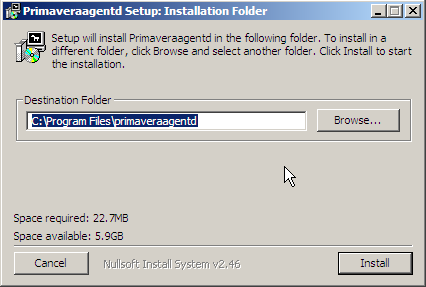
\includegraphics[scale=0.6]{screenshots/primavera/primaverainstall_01.png}
    \caption{Step 1 - Choosing installation directory}
    \label{fig:primavera_install_passo1}
    \end{center}
\end{figure}

\begin{figure}[H]
    \begin{center}
    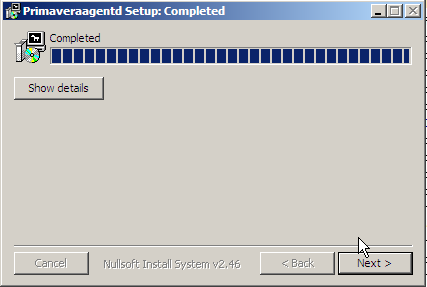
\includegraphics[scale=0.6]{screenshots/primavera/primaverainstall_02.png}
    \caption{Step 2 - Installation progress}
    \label{fig:primavera_install_passo2}
    \end{center}
\end{figure}

\begin{figure}[H]
    \begin{center}
    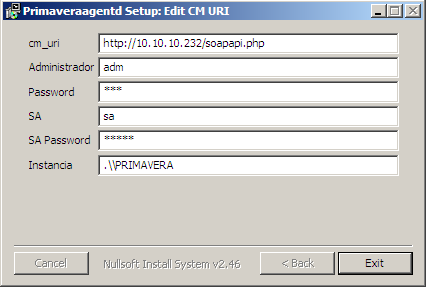
\includegraphics[scale=0.6]{screenshots/primavera/primaverainstall_03.png}
    \caption{Step 3 - Agent setup}
    \label{fig:primavera_install_passo3}
    \end{center}
\end{figure}

In step 3, you need to set some parameters that will allow access to the Primavera's engine thus enabling its management.

\begin{figure}[H]
    \begin{center}
    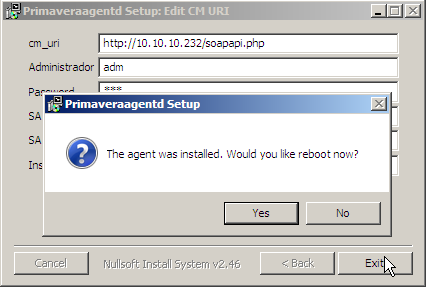
\includegraphics[scale=0.6]{screenshots/primavera/primaverainstall_04.png}
    \caption{Step 4 - Reboot confirmation}
    \label{fig:primavera_install_passo4}
    \end{center}
\end{figure}

\begin{figure}[H]
    \begin{center}
    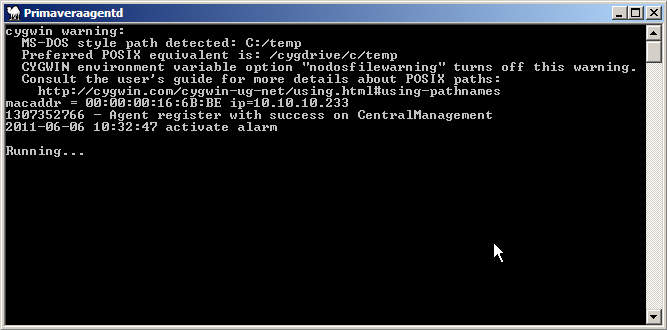
\includegraphics[scale=0.6]{screenshots/primavera/primaverainstall_05.png}
    \caption{Step 5 - Agent startup}
    \label{fig:primavera_install_passo5}
    \end{center}
\end{figure}

After installation is necessary to reboot the virtual machine to initialize the agent.
From this moment you can manage the Primavera service from the Central Management interface.

\subsection{Interface}

The Primavera's management interface allows you to access some essential features for the service's maintenance, including backup management, start and stop operations, manage users and change the IP address of the virtual machine.

\begin{figure}[H]
    \begin{center}
    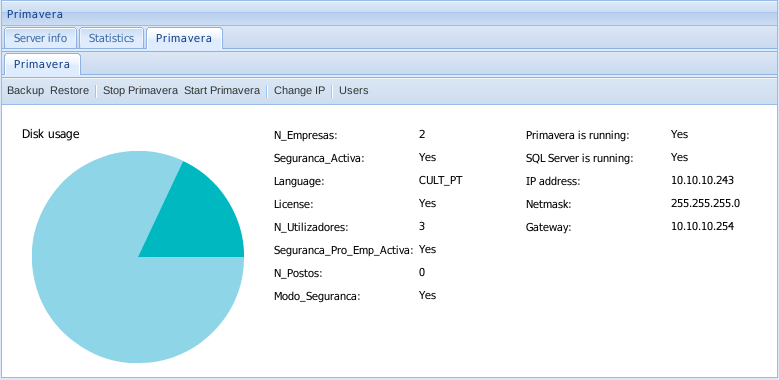
\includegraphics[scale=0.5]{screenshots/primavera/primaverainterface_01.png}
    \caption{Service information}
    \label{fig:primavera_info}
    \end{center}
\end{figure}

When you access the Primavera tab, it's possible to see some information about the service's state such as: disk space usage, number of companies, Primavera's license, number of jobs, state of the Primavera's services and SQL server, and at last the network info.

From the menu bar you can access some other features such as: Backup and restore, start and stop Primavera's service, change network configuration and user management.

\begin{figure}[H]
    \begin{center}
    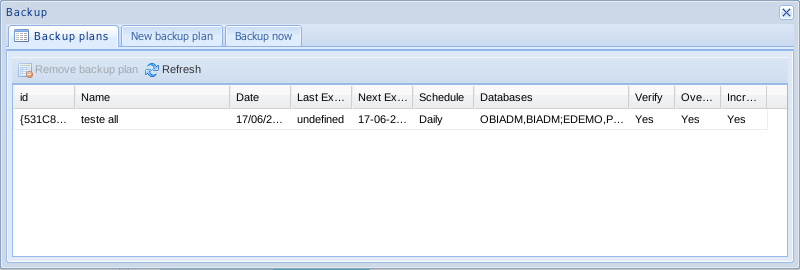
\includegraphics[scale=0.5]{screenshots/primavera/primaverainterface_02.png}
    \caption{Listing backup plans}
    \label{fig:primavera_list_backup_plans}
    \end{center}
\end{figure}

In backup menu we can access the backup feature that allows you to manage backup plans.
To create a new plan, go to the tab \textit{New backup plan} and define the following parameters: \textit{name} - identification of the plan, \textit{frequency} - frequency the backup plan (daily, weekly, monthly), \textit{database} - database that will be carried out \textit{up}, options \textit{check}, \textit{Overwrite} and \textit{Incremental} , set up the plan to check after making \textit{up}, on-call in case of the file already exists and \textit{Incremental backup}.

\begin{figure}[H]
    \begin{center}
    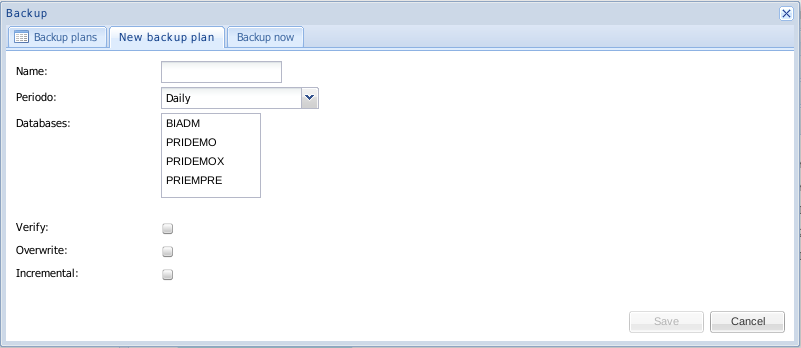
\includegraphics[scale=0.5]{screenshots/primavera/primaverainterface_03.png}
    \caption{Defining a backup plan}
    \label{fig:primavera_new_backup_plan}
    \end{center}
\end{figure}

\begin{figure}[H]
    \begin{center}
    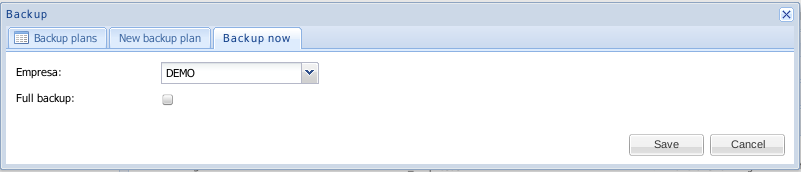
\includegraphics[scale=0.5]{screenshots/primavera/primaverainterface_04.png}
    \caption{Performing a backup}
    \label{fig:primavera_backup_now}
    \end{center}
\end{figure}

There is also the option to make an immediate backup, on tab \textit{Backup now}.
Here we choose the company to make backup or we can perform an entire Primavera's platform backup, choosing the option \textit{Full backup}.

\begin{figure}[H]
    \begin{center}
    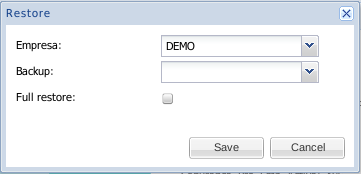
\includegraphics[scale=0.6]{screenshots/primavera/primaverainterface_05.png}
    \caption{Restoring process}
    \label{fig:primavera_restore}
    \end{center}
\end{figure}
In the \textit{Restore} tab we can perform a backup restore.
We can restore a partial backup (for a company), or perform a full Primavera's system restore by selecting the option \textit{Full restore}. 

\begin{figure}[H]
    \begin{center}
    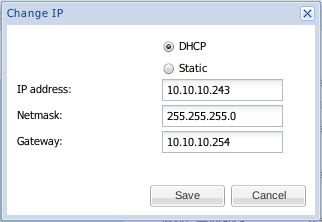
\includegraphics[scale=0.6]{screenshots/primavera/primaverainterface_06.png}
    \caption{Changing the IP address}
    \label{fig:primavera_change_ip}
    \end{center}
\end{figure}

To make change in network configuration we can access the tab \textit{Change IP}, where we can modify the IP address settings, netmask and the gateway of Primavera's virtual machine. 
We can also define the configuration over DHCP.

\begin{figure}[H]
    \begin{center}
    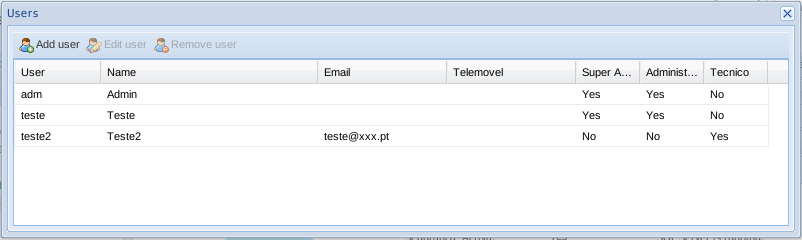
\includegraphics[scale=0.6]{screenshots/primavera/primaverainterface_07.png}
    \caption{List of Primavera's users}
    \label{fig:primavera_list_users}
    \end{center}
\end{figure}

We can manage Primavera's users on tab \textit{Users}.
Here you can list any existing users, configure a new user with several parameters (User Name, Email, and Password options Super Administrator, Administrator and / or technical). It's even possible to edit and user's data or remove users.

\begin{figure}[H]
    \begin{center}
    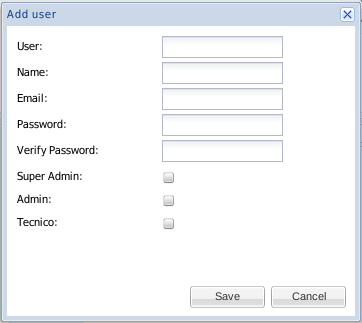
\includegraphics[scale=0.6]{screenshots/primavera/primaverainterface_08.png}
    \caption{Adding a Primavera user}
    \label{fig:primavera_add_user}
    \end{center}
\end{figure}

\begin{figure}[H]
    \begin{center}
    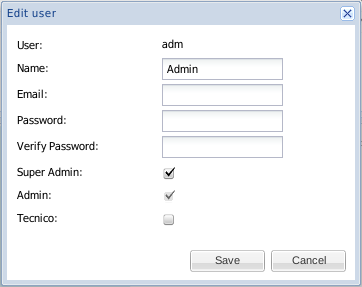
\includegraphics[scale=0.6]{screenshots/primavera/primaverainterface_09.png}
    \caption{Editing a Primavera user}
    \label{fig:primavera_edit_user}
    \end{center}
\end{figure}

\begin{figure}[H]
    \begin{center}
    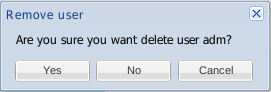
\includegraphics[scale=0.6]{screenshots/primavera/primaverainterface_10.png}
    \caption{Removing a Primavera user}
    \label{fig:primavera_delete_user}
    \end{center}
\end{figure}

